\chapter{Test Hardware}

In this chapter, the features of the target processor used in testing have been described, along with details about how these features were taken into account in simulation. 

\section{Target Processor}
The target processor uses an ARM Cortex A5 core. The salient features are as follows,

\begin{itemize}
\item Single Core Processor
\item In-order Execution Pipeline
\item Dynamic Branch Prediction
\item Separate L1 Cache for Data and Instructions
\item External L2 Cache. Single Cache for Data and Instructions.
\end{itemize}

\subsection{Instruction Pipeline}
The ARM Cortex A5 Core has an 8 stage pipeline. The stages in the pipeline are shown in Figure \ref{fig:pipelineA5}.

%\vspace*{-30pt}
\begin{figure}[h]
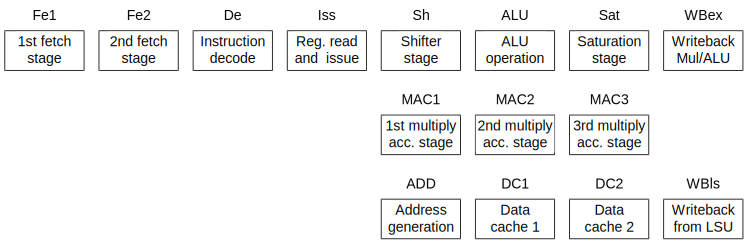
\includegraphics[width=\textwidth]{figures/pipeline.png}
\caption{Pipeline Stages in ARM Cortex A5 Core \cite{CortexA5TRM}}
\label{fig:pipelineA5}
\end{figure}

The first 4 stages are common for all instructions. The next stages are specialized for different types of instructions to reduce interlocking. The Shifter, ALU and Saturation stages are used for Arithmetic and Logical Instructions. The multiplication instruction are executed in 3 multiply accumulate stages. For load store instructions, a separate pipeline is implemented. The pipeline stalls when L1 cache miss occurs and data must be fetched from lower levels of cache or main memory. The result is written back to registers in the last stage.

\subsection{Interlocking}
A strong understanding of interlocking behaviour in the Cortex A5 pipeline is important to estimate the number of cycles spent in execution of each basic block. 

Instructions can have complex dependencies. An accurate estimate of number of cycles spent in execution of instructions is difficult to achieve using static analysis. The ARM Reference Manual \cite{CortexA5TRM} states that for precise timings a cycle-accurate model of the processor must be used. The approach to calculate the cycles spent in pipeline stalls is described here in brief. This approach, if incorrect could introduce inaccuracy in estimation.

For each instruction, the result of the execution will be written to the destination register in the last stage. The next instruction which needs the result will have to wait. To reduce the number of pipeline stalls, results are forwarded to other stages of the pipeline before writing to the register.

\vspace*{-10pt}
\paragraph{Result Latency}
Result Latency is the number of cycles before the result of the instruction is available to be used by the next instruction. 

\begin{Example}
\begin{lstlisting}
LDR R1, [R2]                    ;Result latency three
ADD R3, R3, R1                  ;Register R1 required by ALU
\end{lstlisting}
\end{Example}
\vspace*{-10pt}

For above sequence of instructions, the pipeline will be stalled for 3 cycles.

\vspace*{-10pt}
\paragraph{Early Register}
An Early Register is a register that is needed at the start of Sh, MAC1 or ADD stage (refer to Figure \ref{fig:pipelineA5}) in execution. One more cycle is added to the result latency of the previous instruction producing this register for interlock calculations.

\begin{Example}
\begin{lstlisting}
LDR R1, [R2]                    ;Result latency three
ADD R3, R3, R1    LSL#6         ;plus one, Register R1 is required by Sh
\end{lstlisting}
\end{Example}
\vspace*{-10pt}

In the above example, the value of R1 is needed by the ADD instruction in the Shifter Stage. The pipeline will be stalled for 4 cycles.

\vspace*{-10pt}
\paragraph{Late Register}
A Late Register is not required until the start of the ALU, MAC1 or DC1 stage for the second execution. One cycle is subtracted from the result latency of the previous instruction producing this result for interlock calculations.

\begin{Example}
\begin{lstlisting}
LDR R1, [R2]                    ;Result latency three
ADD R3, R3, R1, R4 LSL#5        ;minus one, Register R1 is a Late Reg
\end{lstlisting}
\end{Example}
\vspace*{-10pt}

In the above example, the pipeline is stalled for only 2 cycles. While the LDR instruction is being executed, the value in R4 is being shifted. After waiting for 2 more cycles, the value of R1 is made available, and execution can proceed.

The binary instructions in each basic block are parsed sequentially. For each instruction, the early and late registers, and corresponding dependencies are identified. Penalties are appropriately added for the pipeline stalls. The results corroborate that the approach is fairly accurate. The accuracy can be further improved by creating a cycle accurate model of the processor pipeline, and simulating the instructions on this model. This will significantly increase the complexity of the approach and the time needed in instrumentation.

\subsection{Branch Prediction Unit}
The Branch Prediction Unit uses algorithm described in Section [TODO] to predict the outcome of a conditional branch instruction. Cortex A5 has a 125 entry Branch History Table. To simulate the effect of Branch Prediction on performance, a branch prediction simulator has been developed.

\subsection{Cache Hierarchy}
\label{sec:c3CacheHierarchy}
ARM Cortex A5 uses separate L1 Cache for Data and Instructions. An interface is provided to use an L2 Cache. On the test setup, an external unified L2 Cache has been used. The parameters of each cache are shown in Table \ref{tbl:cacheSize}. In this section, the details and features of the caches are discussed. 

\vspace*{10pt}
\begin{table}[h]
\centering
%\begin{tabularx}{360pt}{>{\centering\arraybackslash}X>{\centering\arraybackslash}X>{\centering\arraybackslash}X>{\centering\arraybackslash}X}
\begin{tabular}{cccc}
    \toprule
        &  Size   & N-way   & Cache Line Size \\
    \hline
    L1 D Cache  & 32 KB & 4 & 32 B \\
    L1 I Cache  & 32 KB & 2 & 32 B \\
    L2 Cache    & 512 KB & 16 & 32 B \\
    \bottomrule
\end{tabular}
%\end{tabularx}
\caption{Size of Caches}
\label{tbl:cacheSize}
\end{table}

The L1 Caches use a Pseudo Random Replacement Policy, while the L2 Cache used Round Robin Replacement Policy. Cortex A5 uses Exclusive Cache Mode. In this mode, a given address is cached in either L1 Cache or in L2 Cache, but not in both. This has the effect of increasing the usable space and efficiency. The data is loaded from memory into L1 Cache. On eviction from L1, the data is stored in the L2 Cache.

Cortex A5 also supports prefetching of data. The addresses fetched from memory are analyzed and spatial locality of accesses is identified. Data which is highly probable of being used by the application is prefetched in the L1 Cache, thereby saving cycles spent in fetching data from memory.

These features have been implemented in the Cache Simulator to accurately model the Cache. The results corroborate the accuracy in estimation of the number of cache misses occurred. 

%There is a certain error in estimating cycles spent in memory accesses. The Cortex A5 uses a small Store Buffer. Data evicted from L1 cache is buffered in the Store Buffers, and written to L2 Cache in a non-blocking fashion. When the Store Buffer is full, execution is stalled to complete the pending writes to the L2 Cache. This situation is difficult to simulate and account for.

%\subsection{Performance Monitoring Unit}
%ARM Cortex A5 provides a hardware counters which can be used for monitoring various performance parameters. Apart from a cycle counter, two counters are provided which can be programmed to count different types of events. This technique has been used to collect results from actual hardware, and compare with results gathered
